\documentclass[12pt]{article}

\usepackage{geometry} % to change the page dimensions
\geometry{a4paper,hmargin={1in,1in},vmargin={1in,1in}} %
\usepackage[utf8]{inputenc}
\usepackage[vietnam]{babel}
\usepackage{amsmath,amsfonts,amssymb}
\usepackage{color,graphicx,fancybox}
\usepackage{verbatim}
\usepackage{sagetex}


\title{Bài tập nhóm 3 - Phương pháp tính kỹ thuật HK1 2014-2015}
\author{Name: \hspace*{2in}}
\author{Doãn Minh Đăng}
\date{Hạn nộp: 13:30 ngày thứ ba 08/12/2014}


%----------- HEADERS & FOOTERS -------------
\usepackage{fancyhdr} % This should be set AFTER setting up the page geometry
\pagestyle{fancy} % options: empty , plain , fancy
\makeatletter
\let\Title\@title
\let\Author\@author
\let\Date\@date
\makeatother
\fancyhead[LE,RO]{\bfseries\Author}
\fancyhead[RE,LO]{{\Title}}
\usepackage{lastpage}
\cfoot{\thepage\ of \pageref{LastPage}}
\usepackage{hyperref}


%----------- OTHER PACKAGES  -------------
\usepackage{paralist}
\setlength{\pltopsep}{1.5ex}
\setlength{\plitemsep}{0.5ex}
\setdefaultleftmargin{2.5em}{2.2em}{1.87em}{1.7em}{1em}{1em}

\newcommand{\Solution}{
\medskip
{\bf \underline{Lời giải}:}
}

\newcommand{\Collaborators}{
\medskip
{\bf \underline{Collaborators}:}
}

%%% BEGIN DOCUMENT %%%%%%%%%%%%%%%%%%%%%%%

\begin{document}
\thispagestyle{plain}

  \begin{center}%
    {\LARGE \Title \par}%
    \vskip 1.5em%
    {\large  \Author \par}%
      \vskip 1em%
    {\large \Date \par}% 
  \end{center}\par

\section*{Yêu cầu}
\begin{itemize}
 \item Sinh viên có thể ghi kết quả trên giấy viết tay, hoặc đánh máy và in ra. Đối với bài 6 và 7 cần gửi file chương trình cho giảng viên qua email.
 \item Trên bài làm và trên file chương trình, cần ghi cụ thể tên, mã số sinh viên của các thành viên trong nhóm.
 \item Sinh viên làm theo nhóm từ 2 đến 3 thành viên.
 \item Bài nộp trễ sẽ bị trừ 10 điểm cho mỗi ngày trễ hạn.
 \item Câu hỏi số 8 và 9 có bonus, tuy nhiên điểm tối đa cho bài tập nhóm này là 100 điểm, sẽ được quy đổi sang thang điểm 10 khi kết thúc môn học.
\end{itemize}


\section{Bài 1 (10 điểm)}

% Tính tích phân xác định: % độ dài của cung của một hình ellipse
% 
% \begin{align*}
%  \int_{-1}^1 \sqrt{1+\frac{4x^2}{1-x^2}}dx
% \end{align*}

Cho các giá trị rời rạc với $x = 0,1,2,3,4,5,6$, và các giá trị $y$ lần lượt là bằng các chữ số trong mã số sinh viên của bạn (lấy 7 chữ số trong MSSV làm các giá trị $y_0, y_1, \cdots, y_6$). Tính bảng tỉ sai phân theo công thức Newton tiến, và tính giá trị nội suy tại điểm $x=2.5$. Khi báo cáo, cần cho biết vector $y$ mà mình sử dụng để tính toán.

\Solution

Xem kết quả theo mã số sinh viên, ở trang web: 

\url{http://sagecell.sagemath.org/?q=vmjmiz}


\section{Bài 2 (10 điểm)}

Dùng bảng giá trị $x,y$ cho ở Bài 1. Tính gần đúng đạo hàm của các nút phía trong theo công thức sai phân hướng tâm. Khi báo cáo, cần cho biết vector $y$ mà mình sử dụng để tính toán.

\Solution

Xem kết quả theo mã số sinh viên, ở trang web: 

\url{http://sagecell.sagemath.org/?q=thwzbi}

\section{Bài 3 (10 điểm)}

Cho các giá trị rời rạc với $x = 0,2,4,6,8,10,12$, và các giá trị $y$ lần lượt là bằng các chữ số trong mã số sinh viên của bạn (lấy 7 chữ số trong MSSV làm các giá trị $y_0, y_1, \cdots, y_6$). Xem các giá trị này là kết quả của hàm số $y=f(x)$, tính gần đúng tích phân sau theo công thức hình thang:

\begin{align*}
 I = \int_0^{12} f(x) dx
\end{align*}

Khi báo cáo, cần cho biết vector $y$ mà mình sử dụng để tính toán.

\Solution

Xem kết quả theo mã số sinh viên, ở trang web: 

\url{http://sagecell.sagemath.org/?q=bktzkr}

\section{Bài 4 (10 điểm)}

Tìm phương trình đường thẳng xấp xỉ hàm số $f(x)$ với các giá trị $(x,y)$ được cho trong bảng sau, và tính sai số bình phương:

$(0,5)$, $(1,3)$, $(2,3)$, $(3,1)$

%\begin{enumerate}[a)]
%\item $(0,0)$, $(1,3)$, $(2,3)$, $(5,6)$

%\item $(1,2)$,  $(3,2)$,  $(4,1)$,  $(6,3)$

%\item $(0,5)$, $(1,3)$, $(2,3)$, $(3,1)$

%\end{enumerate}

Vẽ đồ thị gồm các điểm được cho và đường thẳng xấp xỉ được. Tính giá trị cực tiểu của phiếm hàm $g(f)=\sum_{k=1}^4 [f(x_k)-y_k]^2$.

\Solution

\begin{sagesilent}
n=4
xk=range(n)
yk=[5,3,3,1]
zk=zip(xk,yk)
plotdata=list_plot(zk, size=50, legend_label='($x_k$,$y_k$)')
xk2=[xk[i]^2 for i in range(n)]
matA=matrix([[n,sum(xk)],[sum(xk),sum(xk2)]])
xkyk=[xk[i]*yk[i] for i in range(n)]
matB=vector([sum(yk),sum(xkyk)])
a,b=N(matA\matB)
a=round(a,4)
b=round(b,4)
hamxapxi=a+b*x
plotline=plot(hamxapxi,0,n, color='red', legend_label='($y=A+Bx$)')

saiso_se=[(hamxapxi(x=xk[i])-yk[i])^2 for i in range(n)]
saiso_sse=sum(saiso_se)

tableVD5=r"\begin{tabular}{l|c|l}"
tableVD5+=r"$k$ & $x_k$ & $y_k$ \\ \hline"
for i in range(n):
  tableVD5+=latex(i) + r"&" + latex(xk[i]) + r"&" + latex(round(yk[i],3)) + r"\\"
tableVD5+=r"\end{tabular}"
\end{sagesilent}

Phương trình đường thẳng xấp xỉ là $y=\sage{hamxapxi(x)}$. Sinh viên cần trình bày được quy trình tính được các tham số của đường thẳng này: xét phương trình đường thẳng $y=A+Bx$, lập hàm số sai số $g(f)=\sum_{k=1}^4 [f(x_k)-y_k]^2$ rồi lấy đạo hàm của $g$ theo $A$ và $B$, cực tiểu của hàm $g$ là ứng với các đạo hàm bằng không, khi đó giải hệ phương trình tuyến tính hai ẩn số đối với $A, B$:
\begin{align*}
\left\lbrace
\begin{array}{l}
 \frac{\partial g}{\partial A} = 0 \\
 \frac{\partial g}{\partial B} = 0
\end{array}\right.
\Leftrightarrow
\left\lbrace
\begin{array}{rcrcl}
 n A &+& \left(\sum_k x_k\right) B &=& \sum_k y_k \\
 \left(\sum_k x_k\right) A &+& \left(\sum_k x_k^2\right) B &=& \sum_k x_k y_k
\end{array}\right.
\end{align*}


Sai số bình phương tức là sai số giữa các giá trị đo và giá trị của hàm số xấp xỉ (tổng sai số bình phương), chính là bằng $g(f)$ ứng với công thức hàm $f=A+Bx=\sage{hamxapxi(x)}$. Tổng sai số bình phương là $SSE = \sage{round(saiso_sse,3)}$.

Dưới đây là tập dữ liệu và đồ thị hàm số xấp xỉ: %\sage{round(a,3)}+\sage{round(b,3)}x$)

\begin{center}
 \begin{tabular}{lc}
   \sagestr{tableVD5}
  & 
    \begin{tabular}{c}
    \sageplot[scale=0.4]{plotdata+plotline}
    \end{tabular}
 \end{tabular} 
\end{center}

Giá trị cực tiểu của phiếm hàm $g(f)=\sum_{k=1}^4 [f(x_k)-y_k]^2$ đạt được tại giá trị $A, B$ mà $\frac{\partial g}{\partial A}=0$ và $\frac{\partial g}{\partial B}=0$. Như đã tính toán ở trước, cực tiểu xảy ra tại $A=\sage{round(a,3)}$ và $B=\sage{round(b,3)}$, và $\min(g)=\sage{round(saiso_sse,3)}$ (cũng bằng với tổng sai số bình phương giữa hàm xấp xỉ và dữ liệu thực).

\section{Bài 5 (20 điểm) $(\star)$}

Tính gần đúng tích phân xác định dưới đây với sai số không vượt quá 0.00001 so với giá trị chính xác, sử dụng bất kỳ phương pháp nào bạn được học. Nêu các bước tính toán và lý giải về sai số.

\[\int_{0}^1  \sin \left( \frac 1 x \right) dx \]

\Solution

\begin{sagesilent}
f(x) = sin(1/x)
plotf1=plot(f,0,1)
plotf2=plot(f,1/(5*pi),1/(2*pi))
f2=diff(f,x,2)
h=0.2*(1/(201*pi)-1/(202*pi))
M2=2*(201*pi)^3+(201*pi)^4
tp_chinhxac=N(integral(f,x,0,1))
#Tính tích phân theo công thức hình thang
def tichphan_trap(f,a=0,b=1,h=0.1):
  n=(b-a)/h
  #chuoif=[f(a+h*i) for i in range(n+1)]
  #tp_trap=h*(sum(chuoif)-0.5*(chuoif[0]+chuoif[n]))
  #return tp_trap
  #Tính kiểu này chậm, vì Sage dùng symbolic math để tính, và khi h nhỏ nó sẽ tốn nhiều bộ nhớ để lưu chuỗi f 
  tp_trap=N(0.5*(f(a)+f(b)))
  for k in range(n):
    tp_trap=tp_trap+N(f(a+h*k))
  tp_trap=h*tp_trap
  return tp_trap
# Áp dụng để tính tích phân I1
tp_1=tichphan_trap(f,1/(202*pi),1/(201*pi),h)
# Áp dụng để tính tích phân I2, sau khi đã xác định được hbar<1.94e-8
hbar=1.9*10^(-6) # tính hết gần 4 phút với Sagetex trên máy laptop Fujitsu-Siemens M9400
tp_2=0.504064437961949
#tp_2=tichphan_trap(f,1/(201*pi),1,hbar) # tính hết gần 4 phút, kết quả: tp_2=0.504064437961949
\end{sagesilent}

Trước tiên, ta xem đồ thị hàm số:

\sageplot[scale=.8]{plotf1}

Việc tính gần đúng tích phân này gặp một số khó khăn như sau:
\begin{itemize}
 \item Hàm số không xác định tại $x=0$, nên các công thức tính gần đúng sẽ bị vướng ở chỗ tính $\sin(\frac{1}{0})$. Tuy $\frac{1}{0}$ không xác định nhưng ta có thể dùng tính chất bị chặn của hàm $\sin$ để vượt qua khó khăn này: $-1 < \sin(\frac{1}{0}) < 1$.
 \item Đây là hàm số $\sin$ mà chu kỳ của nó thay đổi liên tục, càng gần $0$ thì chu kỳ càng ngắn (đòi hỏi bước tính toán càng nhỏ), khi $x$ tăng lên càng gần $1$ thì chu kỳ càng dài lên, độ dài một bước tính toán không đòi hỏi phải quá nhỏ nữa (vì $h$ càng nhỏ thì càng mất công tính toán nhiều). Do đó nếu dùng độ dài bước là $h$ cố định thì tính không tối ưu, mà nên cho $h$ thay đổi.
\end{itemize}

Để tìm được cách tính toán phù hợp, ta quan sát kỹ hơn đồ thị của hàm số $\sin(1/x)$:

%\sageplot[scale=.8]{plotf2}
\begin{center}
 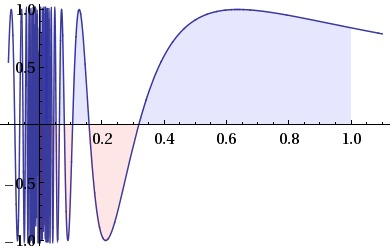
\includegraphics{./integral_sin.jpg}
 % integral_sin.gif: 391x250 pixel, 72dpi, 13.79x8.82 cm, bb=0 0 391 250
\end{center}

Ta thấy tích phân của hàm số này sẽ bao gồm diện tích của các 'nửa chu kỳ' dương trừ cho diện tích của các `nửa chu kỳ' âm (gọi là `nửa chu kỳ' không thực sự đúng về mặt toán học, vì đây không phải là hàm tuần hoàn, ta tạm gọi một `nửa chu kỳ' ở đây là giới hạn giữa hai điểm liền kề nhau mà đồ thị hàm số cắt trục hoành). Hàm số $f(x)=\sin \frac{1}{x}$ cắt trục hoành ($f(x)=0$) tại các điểm sau:

\begin{align*}
 \left\lbrace \begin{array}{l}
               x=\frac{1}{2k \pi}, k \neq 0, k \in \mathbb{Z} \\
               x=\frac{1}{(2k+1) \pi}, k \in \mathbb{Z}
              \end{array}
              \right.
\end{align*}

Với một số tự nhiên $k>0$, thì ta thấy hàm $\sin (\frac{1}{x})$ là dương với $\frac{1}{2k\pi} > x > \frac{1}{(2k+1)\pi}$, và là âm với $\frac{1}{(2k+1)\pi} > x > \frac{1}{(2k+2)\pi}$. Đặt hai dãy số:

\begin{align*}
 d_k &= \int_{\frac{1}{(2k+1)\pi}}^{\frac{1}{2k\pi}} \sin \left( \frac{1}{x} \right) dx > 0, k=1, 2, \cdots \\
 a_k &= - \int_{\frac{1}{2(k+1)\pi}}^{\frac{1}{(2k+1)\pi}} \sin \left( \frac{1}{x} \right) dx > 0, k=1, 2, \cdots
\end{align*}

Giữa các phần diện tích `nửa chu kỳ' có mối quan hệ như sau:

\begin{align}\label{eq_giamdan}
 d_1 > a_1 > d_2 > a_2 > \cdots > d_k > a_k > \cdots > 0
\end{align}

Ta có công thức tính tích phân bằng cách chia ra các khoảng `nửa chu kỳ', với $N>0$ là một số tự nhiên chọn trước:

\begin{align} \label{eq_tichphankhoang}
 \int_{0}^1  \sin \left( \frac 1 x \right) dx &= \int_{\frac{1}{(2N+1)\pi}}^1 \sin \left( \frac{1}{x} \right) -a_{N} + d_{N+1} - a_{N+1} + d_{N+2} - a_{N+2} + \cdots \nonumber \\
 &= \int_{\frac{1}{(2N+1)\pi}}^1 \sin \left( \frac{1}{x} \right) dx -a_{N} + \sum_{k=N+1}^{\infty} (d_k - a_{k})
 \end{align}

Do \eqref{eq_giamdan} nên tổng $\sum_{k=N+1}^{\infty} (d_k-a_{k}) > 0$ và  $\sum_{k=N}^{\infty} (-a_{k-1}+d_k) < 0$, vậy suy ra:
\begin{align}
 &-a_{N} < -a_{N} + \sum_{k=N+1}^{\infty} (d_k - a_{k}) = \sum_{k=N+1}^{\infty} (a_{k-1}+d_k) < 0 \\
 \eqref{eq_tichphankhoang}\Rightarrow &\int_{\frac{1}{(2N+1)\pi}}^1 \sin \left( \frac{1}{x} \right) dx - a_{N} < \int_{0}^1  \sin \left( \frac 1 x \right) dx < \int_{\frac{1}{(2N+1)\pi}}^1 \sin \left( \frac{1}{x} \right) dx \label{eq_chantichphan}
\end{align}

Theo \eqref{eq_chantichphan}, nếu tích phân $a_{N}$ đủ nhỏ thì ta có thể lấy giá trị gần đúng là $\int_{0}^1  \sin \left( \frac 1 x \right) dx \approx \int_{\frac{1}{(2N+1)\pi}}^1 \sin \left( \frac{1}{x} \right) dx$.

Ta sẽ dùng phương pháp tính gần đúng để tính $a_{N} = I_1 \pm \Delta_1$ (với $I_1>0$) và $\int_{\frac{1}{(2N+1)\pi}}^1 \sin \left( \frac{1}{x} \right) dx = I_2 \pm \Delta_2$, khi đó từ biểu thức \eqref{eq_chantichphan}, ta sẽ xác định được xấp xỉ tích phân cần tìm:
\begin{align}
 \int_{0}^1  \sin \left( \frac 1 x \right) dx = I_2 \pm \Delta_I \\
 \textrm{với~} \Delta_I = I_1 + \Delta_1 + \Delta_2 \label{eq_tongsaiso}
\end{align}

Đạo hàm cấp hai của hàm số $f(x)$ là: $f''(x)=\sage{f2(x)}$. Xét trên một đoạn $[a,b]$ với $0<a<b\leq 1$ thì ta có thể ước lượng giá trị cực đại của đạo hàm cấp hai như sau:

\begin{align}\label{eq_uocluongM2}
 M_2 = \max_{x \in [a,b]} |f''(x)| \leq \max_{x \in [a,b]} \left|\frac{2\cos\left(\frac{1}{x}\right)}{x^3}\right| + \max_{x \in [a,b]} \left|\frac{\sin\left(\frac{1}{x}\right)}{x^4}\right| < \max_{x \in [a,b]} \frac{2}{x^3}+\frac{1}{x^4} \leq \frac{2}{a^3}+\frac{1}{a^4}
\end{align}

Lấy $N=100$, ta tính tích phân $a_{N}=a_{100}=-\int_{\frac{1}{202\pi}}^{\frac{1}{201\pi}} \sin \left( \frac{1}{x} \right) dx$ bằng cách chia đoạn đó thành 5 bước, tức là $h=\frac{1}{5} \left(\frac{1}{201\pi}-\frac{1}{202\pi}\right)=\sage{h}$. Ta có:

\begin{align*}
I_1 = -h \left( 0.5f\Big(\frac{1}{202\pi}\Big)+\sum_{k=1}^4 f\Big(\frac{1}{202\pi}+kh\Big)+0.5f\Big(\frac{1}{201\pi}\Big) \right) = \sage{-N(tp_1)}
\end{align*}
với sai số là $\Delta_1 \leq (\frac{1}{201\pi}-\frac{1}{202\pi}) \frac{h^2 M_2}{12} < 
\sage{N((1/(201*pi)-1/(202*pi))*h^2*(2*(202*pi)^3+1*(202*pi)^4)/12)}$.

Tiếp theo, ta tính $I_2$. Để tổng sai số $\Delta_I\leq 10^{-5}$, ta cần tính $I_2$ với sai số $\Delta_2 \leq 10^{-5} - I_1 - \Delta_1$, vậy ta cần đặt mục tiêu $\Delta_2 \leq 4.9 \times 10^{-6}$.

Xét trong khoảng $[a,b]=\left[ \frac{1}{201\pi}, 1 \right]$, theo công thức \eqref{eq_uocluongM2}, ta dùng giá trị chặn trên $M_2 < \frac{2}{a^3}+\frac{1}{a^4} = 2(201\pi)^3+(201\pi)^4 = \sage{N(M2)}$. Gọi $\bar{h}$ là độ dài bước để tính gần đúng tích phân $I_2$ với công thức hình thang, ta tìm $\bar{h}$ bằng cách dùng công thức ước lượng sai số:

\begin{align*}
 \Delta_2 &\leq (b-a)\frac{\bar{h}^2 M_2}{12} \leq 4.9 \times 10^{-6}\\
 \Rightarrow \bar{h} &\leq \sqrt{\frac{4.9 \times 10^{-6}\times 12}{\left(1-\frac{1}{201\pi} \right)M_2}} = \sqrt{\frac{4.9 \times 10^{-6}\times 12}{\sage{N((1-1/(201*pi))*M2)}}} = \sage{N(sqrt(4.9*10^(-6)*12/((1-1/(201*pi))*M2)))}
\end{align*}

Áp dụng phương pháp hình thang để tính tích phân $I_2 = \int_{\frac{1}{201\pi}}^1 \sin \left( \frac{1}{x} \right) dx$ với bước tính $\bar{h}=1.9 \times 10^{-8}$, ta thu được: $I_2 = \sage{tp_2}$.

Vậy, kết quả cuối cùng là:

\begin{align}
\int_{0}^1  \sin \left( \frac 1 x \right) dx = I_2 \pm \Delta_I = \sage{round(tp_2,6)} \pm \Delta_I\\
 \textrm{với~} \Delta_I < 10^{-5} 
\end{align}

So sánh với giá trị chính xác: $\sage{tp_chinhxac}$.

\textbf{Ghi chú:} 
\begin{itemize}
 \item Tích phân $I_2$ cần được tính bằng cách lập trình trên máy tính. 
 \item Nếu muốn tiết kiệm thời gian tính toán, ta có thể lập trình với số bước $\bar{h}$ thay đổi để giảm bớt số đoạn chia nhỏ ($\bar{h}$ tăng dần khi $x$ càng lớn), vì đặc điểm của hàm số $\sin \left(\frac{1}{x}\right)$ là biến đổi chậm dần khi $x$ tăng.
 \item Bước tính $\bar{h}=1.9\times 10^{-8}$ là giá trị tính theo lý thuyết đảm bảo đạt sai số nhỏ hơn $10^{-5}$, thực tế với $\bar{h}=2\times 10^{-6}$ đã đạt được sai số đó.
 \item Phần chứng minh các tích phân `nửa chu kỳ' là bù cho nhau liên tiếp để dẫn đến kết quả \eqref{eq_chantichphan}, thực ra là không quá cần thiết vì nó phụ thuộc vào khả năng quan sát đồ thị và nhận ra mối quan hệ giữa hai dãy $a_k, d_k$ như ở \eqref{eq_giamdan}. Sinh viên có thể chỉ cần chia đoạn $[0,1]$ ra làm hai phần là $[0,\epsilon]$ và $[\epsilon,1]$; trên đoạn $[0,\epsilon]$ với $\epsilon \ll 1$ thì dùng cực đại của hàm số $\sin$ để tính chặn trên của tích phân là $I_1 = \int_{0}^{\epsilon} \sin \left( \frac{1}{x} \right) dx < \int_0^{\epsilon} 1 dx = \epsilon$ và xem đây là một thành phần của sai số tổng hợp giống như ở \eqref{eq_tongsaiso}, rồi tìm bước tính $h$ phù hợp để tính gần đúng tích phân trên đoạn $[\epsilon,1]$ với sai số không quá $10^{-5}-\epsilon$, giống như cách làm ở trên, từ biểu thức \eqref{eq_uocluongM2} trở về sau.
\end{itemize}

\section{Bài 6 (10 điểm)}
Viết một chương trình Octave để thực hiện giải thuật tính đa thức nội suy Lagrange, chương trình nhận ba tham số là các vector $x$ và $y$ cho biết bộ dữ liệu các điểm, và một số $xx$ là điểm mà chương trình cần tính giá trị nội suy (là kết quả đầu ra của chương trình)

Sinh viên nộp chương trình dạng file function \emph{noisuy\_lagrange.m}, file này phải chứa chương trình sao cho có thể gọi nó với cú pháp sau:

yx = noisuy\_lagrange(x,y,xx)

Thử nghiệm chương trình trên với các vector $x, y$ của Bài 1, và $xx=3.5$.

\textbf{Lưu ý}: dựa trên các tham số đầu vào $x, y$, chương trình này cần tự xác định được bộ dữ liệu có bao nhiêu điểm.

\section{Bài 7 (10 điểm)}
Viết một chương trình Octave để tính gần đúng đạo hàm với các giá trị đo đạc của hàm số được cho bằng hai vector $x$ và $y$, theo công thức sai phân tiến ($f'(x_k)=\frac{y_{k+1}-y_k}{x_{k+1}-x_k}$).

Sinh viên nộp chương trình dạng file function \emph{saiphan\_tien.m}, file này phải chứa chương trình sao cho có thể gọi nó với cú pháp sau:

dy = saiphan\_tien(x,y)

Thử nghiệm chương trình trên với các vector $x, y$ của Bài 1.

\section{Bài 8 (10+10 điểm)}
Tìm các ví dụ trong thực tế, trong các môn học khác, về việc cần xấp xỉ một hàm thực nghiệm (từ bảng giá trị $(x_k,y_k)$, tìm hàm số theo một dạng cho trước sao cho sai số bình phương là bé nhất). Trình bày ví dụ đó, cho biết dạng của hàm số cần xấp xỉ (đường thẳng / đường parabol / hàm tuần hoàn...), và nêu ý nghĩa của việc tính được hàm số xấp xỉ đó.

Các nhóm sinh viên không được sao chép ý tưởng của nhau. Nếu có ví dụ được hai hay nhiều nhóm cùng sử dụng, điểm số chỉ được tính cho nhóm nào gửi đầu tiên. Các nhóm có thể gửi giải đáp cho bài 8 này nhiều lần qua email trước khi gửi bài báo cáo cuối cùng cho bài tập nhóm này (để đăng ký ý tưởng mình nghĩ ra).

Mỗi ví dụ đúng đắn và trình bày rõ ràng được tính 5 điểm.

\textbf{Bonus}: Nếu báo cáo bài tập nhóm được hoàn thành kịp hạn chót, thì câu này có thể đạt tối đa 20 điểm. Nếu báo cáo bài tập nhóm được gửi trễ hạn, thì câu này chỉ được tối đa 10 điểm.

\section{Bài 9 (10+10 điểm)}
Tìm các ví dụ trong thực tế, trong các môn học khác, về việc cần tính gần đúng đạo hàm hoặc tích phân xác định (từ bảng giá trị $(x_k,y_k)$). Trình bày ví dụ đó, và nêu ý nghĩa của việc tính được các giá trị đạo hàm / tích phân đó.

Các nhóm sinh viên không được sao chép ý tưởng của nhau. Nếu có ví dụ được hai hay nhiều nhóm cùng sử dụng, điểm số chỉ được tính cho nhóm nào gửi đầu tiên. Các nhóm có thể gửi giải đáp cho bài 9 này nhiều lần qua email trước khi gửi bài báo cáo cuối cùng cho bài tập nhóm này (để đăng ký ý tưởng mình nghĩ ra).

Mỗi ví dụ đúng đắn và trình bày rõ ràng được tính 5 điểm.

\textbf{Bonus}: Nếu báo cáo bài tập nhóm được hoàn thành kịp hạn chót, thì câu này có thể đạt tối đa 20 điểm. Nếu báo cáo bài tập nhóm được gửi trễ hạn, thì câu này chỉ được tối đa 10 điểm.

\end{document}
